\input{mmd6-tufte-book-leader}
\def\mytitle{MultiMarkdown User's Guide}
\def\latextitle{MultiMarkdown \\ User's Guide}
\def\myauthor{Fletcher T. Penney}
\def\version{6.4.0}
\def\revised{2018-11-29}
\def\uuid{88e8f53c-9a02-4e49-a639-f2dbb0a2e338}
\newacronym{MMD}{MMD}{MultiMarkdown}

\newacronym{MD}{MD}{Markdown}

\input{mmd6-tufte-book-begin}

\chapter{MultiMarkdown User's Guide}
\label{title}

\begin{quote}
Version 6.4.0\\
Revised 2018-11-29
\end{quote}

\tableofcontents

\chapter{Introduction}
\label{introduction}

MultiMarkdown is a superset of the \href{http://daringfireball.net/projects/markdown/}{Markdown}\footnote{\href{http://daringfireball.net/projects/markdown/}{http:\slash \slash daringfireball.net\slash projects\slash markdown\slash }} lightweight markup syntax with support for additional output formats and features.

\section{What is Markdown?}
\label{whatismarkdown}

To understand what MultiMarkdown is, you first should be familiar with
\href{http://daringfireball.net/projects/markdown/}{Markdown}\footnote{\href{http://daringfireball.net/projects/markdown/}{http:\slash \slash daringfireball.net\slash projects\slash markdown\slash }}. The best description of what Markdown is comes from John Gruber's
Markdown web site:

\begin{quote}
Markdown is a text-to-HTML conversion tool for web writers. Markdown
allows you to write using an easy-to-read, easy-to-write plain text
format, then convert it to structurally valid XHTML (or HTML).
\end{quote}

\begin{quote}
Thus, ``Markdown'' is two things: (1) a plain text formatting
syntax; and (2) a software tool, written in Perl, that converts
the plain text formatting to HTML. See the Syntax page for details
pertaining to Markdown's formatting syntax. You can try it out,
right now, using the online Dingus.
\end{quote}

\begin{quote}
The overriding design goal for Markdown's formatting syntax is to
make it as readable as possible. The idea is that a Markdown-formatted
document should be publishable as-is, as plain text, without looking
like it's been marked up with tags or formatting instructions. While
Markdown's syntax has been influenced by several existing
text-to-HTML filters, the single biggest source of inspiration for
Markdown's syntax is the format of plain text email. --- \href{http://daringfireball.net/projects/markdown/}{John Gruber}\footnote{\href{http://daringfireball.net/projects/markdown/}{http:\slash \slash daringfireball.net\slash projects\slash markdown\slash }}
\end{quote}

\section{What is MultiMarkdown?}
\label{whatismultimarkdown}

Markdown is great, but it lacked a few features that would allow it to work with entire documents, rather than just pieces of a web page.

I wrote MultiMarkdown in order to leverage Markdown's syntax, but to extend it to work with complete documents that could ultimately be converted from text into other formats, including complete HTML documents, LaTeX, PDF, and ODF.

In addition to the ability to work with complete documents and conversion to formats beyond HTML, the Markdown syntax was lacking a few other things. Michel Fortin added a few additional syntax features when writing \href{http://www.michelf.com/projects/php-markdown/extra/}{PHP Markdown Extra}\footnote{\href{http://www.michelf.com/projects/php-markdown/extra/}{http:\slash \slash www.michelf.com\slash projects\slash php-markdown\slash extra\slash }}. Some of his ideas were implemented and expanded on in MultiMarkdown, including tables, footnotes, citation support, image and link attributes, cross-references, math support, and more.

John Gruber may disagree with me, but I really did try to stick with his proclaimed vision whenever I added a new syntax format to MultiMarkdown. The quality that attracted me to Markdown the most was its clean format. Reading a plain text document written in Markdown is \emph{easy}. It makes sense, and it looks like it was designed for people, not computers. To the extent possible, I tried to keep this same concept in mind when working on MultiMarkdown.

I may or may not have succeeded in this{\ldots}.

In the vein of Markdown's multiple definitions, you can think of MultiMarkdown as:

\begin{enumerate}
\item A program to convert plain text to a fully formatted document.

\item The syntax used in the plain text to describe how to convert it to a complete document.

\end{enumerate}

\section{Why should I use MultiMarkdown?}
\label{whyshouldiusemultimarkdown}

Writing with MultiMarkdown allows you to separate the content and structure of your document from the formatting. You focus on the actual writing, without having to worry about making the styles of your chapter headers match, or ensuring the proper spacing between paragraphs. And with a little forethought, a single plain text document can easily be converted into multiple output formats without having to rewrite the entire thing or format it by hand. Even better, you don't have to write in ``computer-ese'' to create well formatted HTML or LaTeX commands. You just write, MultiMarkdown takes care of the rest.

For example, instead of writing:

\begin{verbatim}
<p>In order to create valid 
<a href="http://en.wikipedia.org/wiki/HTML">HTML</a>, you 
need properly coded syntax that can be cumbersome for 
&#8220;non-programmers&#8221; to write. Sometimes, you
just want to easily make certain words <strong>bold
</strong>, and certain words <em>italicized</em> without
having to remember the syntax. Additionally, for example,
creating lists:</p>

<ul>
<li>should be easy</li>
<li>should not involve programming</li>
</ul>
\end{verbatim}

You simply write:

\begin{verbatim}
In order to create valid [HTML], you need properly
coded syntax that can be cumbersome for 
"non-programmers" to write. Sometimes, you just want
to easily make certain words **bold**, and certain 
words *italicized* without having to remember the 
syntax. Additionally, for example, creating lists:

* should be easy
* should not involve programming

[HTML]: http://en.wikipedia.org/wiki/HTML
\end{verbatim}

Additionally, you can write a MultiMarkdown document in any text editor, on any operating system, and know that it will be compatible with MultiMarkdown on any other operating system and processed into the same output. As a plain text format, your documents will be safe no matter how many times you switch computers, operating systems, or favorite applications. You will always be able to open and edit your documents, even when the version of the software you originally wrote them in is long gone.

These features have prompted several people to use MultiMarkdown in the process of writing their books, theses, and countless other documents.

There are many other reasons to use MultiMarkdown, but I won't get into all of them here.

\emph{By the way} --- the MultiMarkdown web site is, of course, created using MultiMarkdown. To view the \gls{MMD} source for any page, add \texttt{.txt} to the end of the URL. If the URL ends with \texttt{\slash }, then add \texttt{index.txt} to the end instead. The main MultiMarkdown page, for example, would be \href{http://fletcherpenney.net/multimarkdown/index.txt}{http:\slash \slash fletcherpenney.net\slash multimarkdown\slash index.txt}.

\section{What Are the Different Versions of MultiMarkdown?}
\label{whatarethedifferentversionsofmultimarkdown}

The first real version of MultiMarkdown was version 2. It was a modification of the original \texttt{Markdown.pl} script. It worked fine, but was slow when parsing longer documents. The plain text was converted to HTML, and then XSLT was used to convert the HTML to other formats (primarily LaTeX). Over time, maintaining the complicated nest of regular expressions became more difficult, and a better approach was needed.

\href{https://github.com/fletcher/peg-multimarkdown}{MultiMarkdown 3}\footnote{\href{https://github.com/fletcher/peg-multimarkdown}{https:\slash \slash github.com\slash fletcher\slash peg-multimarkdown}} (aka \texttt{peg-multimarkdown}) was built using John MacFarlane's \href{https://github.com/jgm/peg-markdown}{peg-markdown}\footnote{\href{https://github.com/jgm/peg-markdown}{https:\slash \slash github.com\slash jgm\slash peg-markdown}} as a base. It was \emph{much} faster than version 2, and the underlying PEG (parsing expression grammar) made things more reliable. There were still issues and limitations (some inherited from peg-markdown, but most were my errors), which lead to the development of version 4.

\href{http://github.com/fletcher/MultiMarkdown-4}{MultiMarkdown 4}\footnote{\href{http://github.com/fletcher/MultiMarkdown-4}{http:\slash \slash github.com\slash fletcher\slash MultiMarkdown-4}} was a complete rewrite, keeping only the PEG and a few utility routines from \gls{MMD} v3. This release fixed memory leaks and other problems from earlier \gls{MMD} releases; it is safe to use in multithreaded applications and adds many new features.

\href{http://github.com/fletcher/MultiMarkdown-5}{MultiMarkdown 5}\footnote{\href{http://github.com/fletcher/MultiMarkdown-5}{http:\slash \slash github.com\slash fletcher\slash MultiMarkdown-5}} was mostly a restructuring of version 4, followed by further incremental improvements.

\href{http://github.com/fletcher/MultiMarkdown-6}{MultiMarkdown 6}\footnote{\href{http://github.com/fletcher/MultiMarkdown-6}{http:\slash \slash github.com\slash fletcher\slash MultiMarkdown-6}} was a complete rewrite from the ground up. The primary goals were:

\begin{itemize}
\item Improved performance -- v6 uses a parser that was largely written by hand, combined with a few pieces that are generated by \href{http://www.hwaci.com/sw/lemon/}{lemon}\footnote{\href{http://www.hwaci.com/sw/lemon/}{http:\slash \slash www.hwaci.com\slash sw\slash lemon\slash }}. This is vastly faster than the PEG parser of versions 3--5. There is probably still room to improve the code, but v6 is now almost as fast as the fastest Markdown parsers out there, \emph{and} provides more features.

\item Improved accuracy and consistency -- v6 uses an entirely new test suite in order to ensure more consistent parsing across various edge cases.

\item New features -- several features were added to v6, and several were completely restructured to provide various improvements.

\item The v6 \href{https://github.com/fletcher/MultiMarkdown-6/tree/master/QuickStart}{QuickStart guide}\footnote{\href{https://github.com/fletcher/MultiMarkdown-6/tree/master/QuickStart}{https:\slash \slash github.com\slash fletcher\slash MultiMarkdown-6\slash tree\slash master\slash QuickStart}} documents some of the changes in this latest iteration.

\end{itemize}

\section{Where is this Guide Kept?}
\label{whereisthisguidekept}

This guide has been rewritten with the following changes:

\begin{itemize}
\item The source is now in the \texttt{gh\_pages} branch of the \href{https://github.com/fletcher/MultiMarkdown-6}{MultiMarkdown project}\footnote{\href{https://github.com/fletcher/MultiMarkdown-6}{https:\slash \slash github.com\slash fletcher\slash MultiMarkdown-6}}. You can submit changes as a pull request, or by writing me.

\item You can access this information on the web at \href{http://fletcher.github.io/MultiMarkdown-5}{http:\slash \slash fletcher.github.io\slash MultiMarkdown-5}

\item The source itself is a collection of MultiMarkdown text documents that use the transclusion features to create a master document from the individual source files. These documents can be viewed in the browser as HTML, or downloaded as PDF or OpenDocument files.

\end{itemize}

\chapter{Usage}
\label{usage}

\section{Basic Command Line Usage}
\label{basiccommandlineusage}

First, verify that you have properly installed MultiMarkdown:

\begin{verbatim}
multimarkdown --version
multimarkdown --v
\end{verbatim}

To learn more about the command line options available:

\begin{verbatim}
multimarkdown --help
multimarkdown --h
\end{verbatim}

To convert a file to HTML:

\begin{verbatim}
multimarkdown file.txt
\end{verbatim}

To save the HTML to a file

\begin{verbatim}
multimarkdown file.txt > file.html
\end{verbatim}

To convert to a different format:

\begin{verbatim}
multimarkdown -t latex file.txt
multimarkdown -t epub file.txt
\end{verbatim}

\section{Batch Mode}
\label{batchmode}

Batch mode allows you to convert one or more files in a single command, saving each file to a separate output file with a file extension based on the output format (e.g. \texttt{.html} or \texttt{.tex}). This will overwrite existing files.

\begin{verbatim}
multimarkdown -b file.txt file2.txt
\end{verbatim}

\section{Transclusion Only}
\label{transclusiononly}

You can output to the \texttt{mmd} format to perform file transclusion and then output the raw \gls{MMD} source before converting to another format:

\begin{verbatim}
multimarkdown -t mmd file.txt
\end{verbatim}

\section{Convenience Scripts}
\label{conveniencescripts}

There are several convenience scripts to batch convert to a specified format:

\begin{verbatim}
mmd file.txt
markdown file.txt		// Compatibility mode
mmd2epub file.txt
mmd2fodt file.txt
mmd2odt file.txt
mmd2opml file.txt
mmd2pdf file.txt		// Convert to LaTeX and process to PDF
mmd2tex file.txt
\end{verbatim}

\section{Advanced Options}
\label{advancedoptions}

\begin{verbatim}
multimarkdown -f, multimarkdown --full
multimarkdown -s, multimarkdown --snippet
\end{verbatim}

Control whether MultiMarkdown outputs a complete document or just a ``snippet''. A snippet includes just the section of text included in the document. A full\slash complete document includes header information and other structure to form a complete HTML or LaTeX document, for example. Additionally, if metadata is included (with a few exceptions), MultiMarkdown will automatically produce a complete document.

\begin{verbatim}
multimarkdown -c, multimarkdown --compatibility
\end{verbatim}

Compatibility mode forces MultiMarkdown to create HTML that matches the output of basic Markdown. In other words, it disables all the new features added in MultiMarkdown.

There are a few exceptions, however. The original \texttt{Markdown.pl} script used recursive regular expressions to perform parsing. This is very flexible (though error-prone), but is extremely slow. MultiMarkdown v6 has a \emph{much} faster parser, but there is one key limitation -- it parses in order and can't look ahead indefinitely to see what might be coming up. The main situations where this occurs is in handling fenced code blocks (not a problem in compatibility mode, since they don't exist in Markdown) and in handling raw HTML. For more information on this, see \href{https://github.com/fletcher/MultiMarkdown-6/issues/135}{https:\slash \slash github.com\slash fletcher\slash MultiMarkdown-6\slash issues\slash 135}.

The other potential difference is that MultiMarkdown v6 has a smarter strong\slash emphasis parser than \texttt{Markdown.pl} -- it better handles edge cases.

Because of these exceptions, there may be a few rare situations where the output generated by MultiMarkdown v6 does not match that by \texttt{Markdown.pl}. If you find what you believe to be a bug that doesn't fit one of these situations, please let me know and I'll take a look. The goal is to match the original Markdown output as much as possible, but not to match the many bugs that are contained in \texttt{Markdown.pl}.

\begin{verbatim}
multimarkdown --random
\end{verbatim}

Normally MultiMarkdown assigns consecutive numbers to the identifiers used for footnotes, citations, etc. (e.g. 1, 2, 3, etc.) This means that you have a ``blog-style'' web site that shows multiple articles on the home page, and multiple stories have footnotes, the anchors will collide. The \texttt{random} option generates random anchor numbers to dramatically reduce the offs of a collision.

\begin{verbatim}
multimarkdown --unique
\end{verbatim}

The \texttt{unique} option uses a similar random number generator to provide unique anchors (``labels'') for headers that do not have a manually specified label. This prevents every ``Introduction'' header in a textbook, for example, from having the identical label \texttt{\#introduction}. This reduces validation errors in HTML, ePub, and LaTeX, and prevents collisions when using the \texttt{\{\{TOC\}\}} function.

\begin{verbatim}
multimarkdown --nosmart
\end{verbatim}

Disable smart quotes (e.g. \texttt{"foo"} does not become \texttt{“foo”}).

\begin{verbatim}
multimarkdown --nolabels
\end{verbatim}

Disables automatic generation of labels\slash anchors for headers.

\begin{verbatim}
multimarkdown --notransclude
\end{verbatim}

Disables file transclusion that allows inserting the contents of a file inside another file. See the section on File Transclusion (\autoref{filetransclusion}) for more information.

\begin{verbatim}
multimarkdown --opml
\end{verbatim}

Allows MultiMarkdown to read an \href{https://en.wikipedia.org/wiki/OPML}{OPML}\footnote{\href{https://en.wikipedia.org/wiki/OPML}{https:\slash \slash en.wikipedia.org\slash wiki\slash OPML}} source file. Outline Processor Markup Language is an XML file format commonly used for outliners and mind mapping programs. MultiMarkdown can read\slash write to this format in addition to using regular plain text files.

\begin{verbatim}
multimarkdown --itmz
\end{verbatim}

Similar to OPML, ITMZ is an outlining format specific to the \href{https://www.toketaware.com/}{iThoughts}\footnote{\href{https://www.toketaware.com/}{https:\slash \slash www.toketaware.com\slash }} mind-mapping program. I added this format because:

\begin{enumerate}
\item iThoughts is my preferred mind-mapping tool

\item iThoughts supports OPML, but the support is (unfortunately) limited. I was unable to convince the author of the benefits of better read\slash write support for OPML.

\item Adding ITMZ support after adding OPML support wasn't that hard.

\item Adding ITMZ support to MultiMarkdown allows me to do some interesting things in MultiMarkdown Composer, as well as in other workflows. (More to come on that.)

\end{enumerate}

Though I reluctantly added support for this format to MultiMarkdown, I will not be adding support for a laundry list of other formats. Plain text and OPML should be enough. If the use of these outline file formats for MultiMarkdown (or regular Markdown) continues to gain traction, then hopefully other developers will include proper OPML support in their programs.

As an aside, the first use of this functionality came when I created an export plug-in for \href{https://www.omnigroup.com/omnioutliner/}{OmniOutliner}\footnote{\href{https://www.omnigroup.com/omnioutliner/}{https:\slash \slash www.omnigroup.com\slash omnioutliner\slash }} that created a plain Markdown\slash MultiMarkdown text file when exporting from an Omnioutliner OPML file.

\begin{verbatim}
multimarkdown -t, multimarkdown --to=FORMAT
\end{verbatim}

Specify the output format.

\begin{verbatim}
multimarkdown -o, multimarkdown --output=FILE
\end{verbatim}

Specify the output file name.

\begin{verbatim}
multimarkdown -a, multimarkdown --accept
multimarkdown -r, multimarkdown --reject
\end{verbatim}

Either accept or reject all proposed \href{http://criticmarkup.com/}{CriticMarkup}\footnote{\href{http://criticmarkup.com/}{http:\slash \slash criticmarkup.com\slash }} changes contained within the document before processing. It basically allows you to output a ``before'' and an ``after'' version of a document containing edits. If neither option is used, MultiMarkdown attempts to show the edits in-line, but this is not always possible for poorly structured edits. See the section on \href{http://criticmarkup.com/}{Criticmarkup}\footnote{\href{http://criticmarkup.com/}{http:\slash \slash criticmarkup.com\slash }} for more information.

\begin{verbatim}
multimarkdown -l, multimarkdown --lang=LANG
\end{verbatim}

Localize language\slash smart quotes for \texttt{en, es, de, fr, he, nl, sv}. This can also be controlled via metadata.

\begin{verbatim}
multimarkdown -m, multimarkdown --metadata-keys
\end{verbatim}

List all metadata keys contained in the document.

\begin{verbatim}
multimarkdown -e, multimarkdown --extract=KEY
\end{verbatim}

Extract the value of a specified metadata key. This is useful for custom scripts, for example.

\chapter{Syntax}
\label{syntax}

\section{Abbreviations (or Acronyms)}
\label{abbreviationsoracronyms}

\textbf{NOTE}: The syntax for abbreviations changed in \gls{MMD} v6.

Abbreviations can be specified using inline or reference syntax. The inline variant requires that the abbreviation be wrapped in parentheses and immediately follows the \texttt{>}.

\begin{verbatim}
[>MMD] is an abbreviation.  So is [>(MD) Markdown].

[>MMD]: MultiMarkdown
\end{verbatim}

There is also a ``shortcut'' method for abbreviations that is similar to the approach used in prior versions of \gls{MMD}. You specify the definition for the abbreviation in the usual manner, but \gls{MMD} will automatically identify each instance where the abbreviation is used and substitute it automatically. In this case, the abbreviation is limited to a more basic character set which includes letters, numbers, periods, and hyphens, but not much else. For more complex abbreviations, you must explicitly mark uses of the abbreviation.

There are a few limitations:

\begin{itemize}
\item The full name of the abbreviation is plain text only -- no MultiMarkdown markup will be processed.

\item When exporting to LaTeX, the \texttt{acronym} package is used; this means that the first usage will result in \texttt{full text (short)}, and subsequent uses will result in \texttt{short}.

\end{itemize}

\section{Citations}
\label{citations}

I have included support for \emph{basic} bibliography features in MultiMarkdown. I'm open to feedback on ways to improve this but keep the following in mind:

\begin{enumerate}
\item Bibliography support in MultiMarkdown is rudimentary. The goal is to offer a basic standalone feature, that can be changed using the tool of your choice to a more robust format (e.g. BibTeX, CiteProc).

\item Those needing more detailed function sets for their bibliographies may need customized tools to provide those services. This is a basic tool that should work for most people. Reference librarians, for example, will probably not be satisfied.

\end{enumerate}

To use citations in MultiMarkdown, you use a syntax much like that for links:

\begin{verbatim}
This is a statement that should be attributed to
its source[p. 23][#Doe:2006].

And following is the description of the reference to be
used in the bibliography.

[#Doe:2006]: John Doe. *Some Big Fancy Book*.  Vanity Press, 2006.
\end{verbatim}

You are not required to use a locator (e.g. ``p. 23''), and there are no special rules on what can be used as a locator if you choose to use one. If you prefer to omit the locator, just use an empty set of square brackets before the citation:

\begin{verbatim}
This is a statement that should be attributed to its 
source[][#Doe:2006].
\end{verbatim}

There are no rules on the citation key format that you use (e.g. \texttt{Doe:2006}), but it must be preceded by a \texttt{\#}, just like footnotes use \texttt{\^{}}.

As for the reference description, you can use Markup code within this section, and I recommend leaving a blank line afterwards to prevent concatenation of several references. Note that there is no way to reformat these references in different bibliography styles; for this you need a program designed for that purpose (e.g. BibTeX).

If you want to include a source in your bibliography that was not cited, you may use the following:

\begin{verbatim}
[Not cited][#citekey]
\end{verbatim}

The \texttt{Not cited} bit is case insensitive.

If you are creating a LaTeX document, the citations will be included, and natbib will be used by default. If you are not using BibTeX and are getting errors about your citations not being compatible with `Author-Year', you can add the following to your documents metadata:

\begin{verbatim}
latex input:	mmd-natbib-plain
\end{verbatim}

This changes the citation style in natbib to avoid these errors, and is useful when you include your citations in the MultiMarkdown document itself.

\textbf{NOTE}: As of version 6, HTML wraps citation references in parentheses instead of brackets, e.g. \texttt{(1)} instead of \texttt{[1]}. Also, citations are now displayed in a separate section from footnotes when outputting to HTML.

\subsection{Inline Citations}
\label{inlinecitations}

Citations can also be used in an inline syntax, just like inline footnotes:

\begin{verbatim}
As per Doe.[#John Doe. *A Totally Fake Book 1*.  Vanity Press, 2006.]
\end{verbatim}

\subsection{BibTeX Citations}
\label{bibtexcitations}

If you are creating a LaTeX document, and need a bibliography, then you should definitely look into \href{http://www.bibtex.org/}{BibTeX}\footnote{\href{http://www.bibtex.org/}{http:\slash \slash www.bibtex.org\slash }} and \href{http://merkel.zoneo.net/Latex/natbib.php}{natbib}\footnote{\href{http://merkel.zoneo.net/Latex/natbib.php}{http:\slash \slash merkel.zoneo.net\slash Latex\slash natbib.php}}. It is beyond the scope of this document to describe how these two packages work, but it is possible to combine them with MultiMarkdown.

To use BibTeX in a MultiMarkdown document, you \emph{must} use the \texttt{BibTeX} metadata (\autoref{bibtex}) to specify where your citations are stored. You may \emph{optionally} use the \texttt{biblio style} metadata key.

Since \texttt{natbib} is enabled by default, you have a choice between using the \texttt{\textbackslash{}citep} and \texttt{\textbackslash{}citet} commands. The following shows how this relates to the MultiMarkdown syntax used.

\begin{verbatim}
[#citekey]    => ~\citep{citekey}
[#citekey][]  => ~\citep{citekey}

[foo][#citekey] => ~\citep[foo]{citekey}

[foo\]\[bar][#citekey] => ~\citep[foo][bar]{citekey}


[#citekey;]    => \citet{citekey}
[#citekey;][]  => \citet{citekey}

[foo][#citekey;] => \citet[foo]{citekey}

[foo\]\[bar][#citekey;] => \citet[foo][bar]{citekey}
\end{verbatim}

\section{CriticMarkup}
\label{criticmarkup}

\subsection{What Is CriticMarkup?}
\label{whatiscriticmarkup}

\begin{quote}
CriticMarkup is a way for authors and editors to track changes to documents in plain text. As with Markdown, small groups of distinctive characters allow you to highlight insertions, deletions, substitutions and comments, all without the overhead of heavy, proprietary office suites. \href{http://criticmarkup.com/}{http:\slash \slash criticmarkup.com\slash }
\end{quote}

CriticMarkup is integrated with MultiMarkdown itself, as well as \href{http://multimarkdown.com/}{MultiMarkdown Composer}\footnote{\href{http://multimarkdown.com/}{http:\slash \slash multimarkdown.com\slash }}. I encourage you to check out the \href{http://criticmarkup.com/}{CriticMarkup}\footnote{\href{http://criticmarkup.com/}{http:\slash \slash criticmarkup.com\slash }} web site to learn more as it can be a very useful tool. There is also a great video showing CriticMarkup in use while editing a document in MultiMarkdown Composer.

\subsection{Using CriticMarkup With MultiMarkdown}
\label{usingcriticmarkupwithmultimarkdown}

When using CriticMarkup with MultiMarkdown itself, you have three choices:

\begin{itemize}
\item Leave the CriticMarkup syntax in place (\texttt{multimarkdown foo.txt}). MultiMarkdown will attempt to show the changes as highlights in the exported document, where possible. This will not \emph{always} result in a valid output document.

\item Accept all changes, giving you the ``new'' document (\texttt{multimarkdown -a foo.txt} or \texttt{multimarkdown -{}-accept foo.txt})

\item Reject all changes, giving you the ``original'' document (\texttt{multimarkdown -r foo.txt} or \texttt{multimarkdown -{}-reject foo.txt})

\item CriticMarkup comments and highlighting are ignored when processing with \texttt{-{}-accept} or \texttt{-{}-reject}.

\end{itemize}

\subsection{The CriticMarkup Syntax}
\label{thecriticmarkupsyntax}

The CriticMarkup syntax is fairly straightforward. The key thing to remember is that CriticMarkup is processed \emph{before} any other MultiMarkdown is handled. It's almost like a separate layer on top of the MultiMarkdown syntax.

When editing in MultiMarkdown Composer, you can have CriticMarkup syntax flagged in the both the editor pane and the preview window. This will allow you to see changes in the HTML preview.

\begin{itemize}
\item Deletions from the original text:

\begin{verbatim}
This is {--is --}a test.
\end{verbatim}

This is \sout{is }a test.

\item Additions:

\begin{verbatim}
This {++is ++}a test.
\end{verbatim}

This \underline{is }a test.

\item Substitutions:

\begin{verbatim}
This {~~isn't~>is~~} a test.
\end{verbatim}

This \sout{isn't}\underline{is} a test.

\item Highlighting:

\begin{verbatim}
This is a {==test==}.
\end{verbatim}

This is a \hl{test}.

\item Comments:

\begin{verbatim}
This is a test{>>What is it a test of?<<}.
\end{verbatim}

This is a test\cmnote{What is it a test of?}.

\end{itemize}

\subsection{CriticMarkup Limitations}
\label{criticmarkuplimitations}

If you \texttt{-{}-accept} or \texttt{-{}-reject} CriticMarkup changes, then it should work properly in any document.

If you want to try to include your changes as ``notes'' in the final document, then certain situations will lead to results that were probably not what you intended.

\begin{enumerate}
\item CriticMarkup must be contained within a single block (e.g. paragraph, list item, etc.) CM that spans multiple blocks will not be recognized.

\item CriticMarkup that crosses multiple \gls{MMD} spans (e.g. \texttt{\{++** foo\} bar**}) will not properly manage the intended MultiMarkdown markup. This example would not result in bold being applied to \texttt{foo bar}.

\end{enumerate}

\subsection{My philosophy on CriticMarkup}
\label{myphilosophyoncriticmarkup}

I view CriticMarkup as two things (in addition to the actual tools that implement these concepts):

\begin{enumerate}
\item A syntax for documenting editing notes and changes, and for collaborating amongst coauthors.

\item A means to display those notes\slash changes in the HTML output.

\end{enumerate}

I believe that \#1 is a really great idea, and well implemented. \#2 is not so well implemented, largely due to the ``orthogonal'' nature of CriticMarkup and the underlying Markdown syntax.

CM is designed as a separate layer on top of Markdown\slash MultiMarkdown. This means that a Markdown span could, for example, start in the middle of a CriticMarkup structure, but end outside of it. This means that an algorithm to properly convert a CM\slash Markdown document to HTML would be quite complex, with a huge number of edge cases to consider. I've tried a few (fairly creative, in my opinion) approaches, but they didn't work. Perhaps someone else will come up with a better solution, or will be so interested that they put the work in to create the complex algorithm. I have no current plans to do so.

Additionally, there is a philosophical distinction between documenting editing notes, and using those notes to produce a ``finished'' document (e.g. HTML or PDF) that keeps those editing notes intact (e.g. strikethroughs, highlighting, etc.) I believe that CM is incredibly useful for the editing process, but am less convinced for the output process (I know many others disagree with me, and that's ok. And to be clear, I think that what Gabe and Erik have done with CriticMarkup is fantastic!)

There are other CriticMarkup tools besides MultiMarkdown and \href{http://multimarkdown.com/}{MultiMarkdown Composer}\footnote{\href{http://multimarkdown.com/}{http:\slash \slash multimarkdown.com\slash }}, and you are more than welcome to use them.

For now, the \emph{official} MultiMarkdown support for CriticMarkup consists of:

\begin{enumerate}
\item CriticMarkup syntax is ``understood'' by the MultiMarkdown parser, and by MultiMarkdown Composer syntax highlighting.

\item When converting from MultiMarkdown text to an output format, you can ignore CM formatting with \texttt{compatibility} mode (probably not what you want to do), accept all changes, or reject all changes (as above). These are the preferred choices.

\item The secondary choice, is to \emph{attempt} to show the changes in the exported document. Because the syntaxes are orthogonal, this will not always work properly, and will not always give valid output files.

\end{enumerate}

\section{Cross-References}
\label{cross-references}

An oft-requested feature was the ability to have Markdown automatically handle
within-document links as easily as it handled external links. To this aim, I
added the ability to interpret \texttt{[Some Text][]} as a cross-link, if a header
named ``Some Text'' exists.

As an example, \texttt{[Metadata][]} will take you to the
section describing metadata (\autoref{metadata}).

Alternatively, you can include an optional label of your choosing to help
disambiguate cases where multiple headers have the same title:

\begin{verbatim}
### Overview [MultiMarkdownOverview] ##
\end{verbatim}

This allows you to use \texttt{[MultiMarkdownOverview]} to refer to this section
specifically, and not another section named \texttt{Overview}. This works with atx-
or settext-style headers.

If you have already defined an anchor using the same id that is used by a
header, then the defined anchor takes precedence.

In addition to headers within the document, you can provide labels for images
and tables which can then be used for cross-references as well.

\section{Definition Lists}
\label{definitionlists}

MultiMarkdown has support for definition lists using the same syntax used in
\href{http://www.michelf.com/projects/php-markdown/extra/}{PHP Markdown Extra}\footnote{\href{http://www.michelf.com/projects/php-markdown/extra/}{http:\slash \slash www.michelf.com\slash projects\slash php-markdown\slash extra\slash }}. Specifically:

\begin{verbatim}
Apple
:	Pomaceous fruit of plants of the genus Malus in 
	the family Rosaceae.
:	An american computer company.

Orange
:	The fruit of an evergreen tree of the genus Citrus.
\end{verbatim}

becomes:

\begin{quote}
\begin{description}
\item[Apple]

 Pomaceous fruit of plants of the genus Malus in
the family Rosaceae.

 An american computer company.

\item[Orange]

 The fruit of an evergreen tree of the genus Citrus.
\end{description}
\end{quote}

You can have more than one term per definition by placing each term on a
separate line. Each definition starts with a colon, and you can have more than
one definition per term. You may optionally have a blank line between the last
term and the first definition.

Definitions may contain other block level elements, such as lists,
blockquotes, or other definition lists.

Unlike PHP Markdown Extra, all definitions are wrapped in \texttt{<p>} tags. First, I
was unable to get Markdown \emph{not} to create paragraphs. Second, I didn't see
where it mattered - the only difference seems to be aesthetic, and I actually
prefer the \texttt{<p>} tags in place. Let me know if this is a problem.

See the \href{http://www.michelf.com/projects/php-markdown/extra/}{PHP Markdown Extra}\footnote{\href{http://www.michelf.com/projects/php-markdown/extra/}{http:\slash \slash www.michelf.com\slash projects\slash php-markdown\slash extra\slash }} page for more information.

\section{Escaped newlines}
\label{escapednewlines}

Thanks to a contribution from \href{https://github.com/njmsdk}{Nicolas}\footnote{\href{https://github.com/njmsdk}{https:\slash \slash github.com\slash njmsdk}}, MultiMarkdown has an additional syntax to indicate a line break. The usual approach for Markdown is ``space-space-newline'' --- two spaces at the end of the line. For some users, this causes problems:

\begin{itemize}
\item the trailing spaces are typically invisible when glancing at the source, making it easy to overlook them

\item some users' text editors modify trailing space (IMHO, the proper fix for this is a new text editor{\ldots})

\end{itemize}

Nicolas submitted a patch that enables a new option that interprets ``\textbackslash{}'' before a newline as a marker that a line break should be used:

\begin{verbatim}
This is a line.\
This is a new line.
\end{verbatim}

\section{Fenced Code Blocks}
\label{fencedcodeblocks}

In addition to the regular indented code block that Markdown uses, you can use ``fenced'' code blocks in MultiMarkdown. These code blocks do not have to be indented, and can also be configured to be compatible with a third party syntax highlighter. These code blocks should begin with 3 to 5 backticks, an optional language specifier (if using a syntax highlighter), and should end with the same number of backticks you started with:

\begin{verbatim}
```perl
# Demonstrate Syntax Highlighting if you link to highlight.js #
# http://softwaremaniacs.org/soft/highlight/en/
print "Hello, world!\n";
$a = 0;
while ($a < 10) {
print "$a...\n";
$a++;
}
```
\end{verbatim}

\begin{lstlisting}[language=perl]
# Demonstrate Syntax Highlighting if you link to highlight.js #
# http://softwaremaniacs.org/soft/highlight/en/
print "Hello, world!\n";
$a = 0;
while ($a < 10) {
print "$a...\n";
$a++;
}
\end{lstlisting}

I don't recommend any specific syntax highlighter, but have used the following metadata to set things up. It may or may not work for you:

\begin{verbatim}
html header:	<link rel="stylesheet" href="http://yandex.st/highlightjs/7.3/styles/default.min.css">
	<script src="http://yandex.st/highlightjs/7.3/highlight.min.js"></script>
	<script>hljs.initHighlightingOnLoad();</script>
\end{verbatim}

Fenced code blocks are particularly useful when including another file (File Transclusion (\autoref{filetransclusion})), and you want to show the \emph{source} of the file, not what the file looks like when processed by MultiMarkdown.

\textbf{NOTE}: In MultiMarkdown v6, if there is no closing fence, then the code block continues until the end of the document.

\section{File Transclusion}
\label{filetransclusion}

File transclusion is the ability to tell MultiMarkdown to insert the contents of another file inside the current file being processed. For example:

\begin{verbatim}
This is some text.

{{some_other_file.txt}}

Another paragraph
\end{verbatim}

If a file named \texttt{some\_other\_file.txt} exists, its contents will be inserted inside of this document \emph{before} being processed by MultiMarkdown. This means that the contents of the file can also contain MultiMarkdown formatted text.

If you want to display the \emph{contents} of the file without processing it, you can include it in a code block (you may need to remove trailing newlines at the end of the document to be included):

\begin{verbatim}
This is some text

```
{{relative/path/to/some_other_file.txt}}
```

Another paragraph
\end{verbatim}

Transclusion is recursive, so the file being inserted will be scanned to see if it references any other files.

Metadata in the file being inserted will be ignored. This means that the file can contain certain metadata when viewed alone that will not be included when the file is transcluded by another file.

You can use the \texttt{[Transclude Base]} metadata to specify where MultiMarkdown should look for the files to be included. All files must be in this folder. If this folder is not specified, then MultiMarkdown will look in the same folder as the parent file.

\textbf{Note:} Thanks to David Richards for his ideas in developing support for this feature.

\subsection{Search Paths}
\label{searchpaths}

When you process a file with \gls{MMD}, it uses that file's directory as the search
path for included files. For example:

\begin{table}[htbp]
\begin{minipage}{\linewidth}
\setlength{\tymax}{0.5\linewidth}
\centering
\small
\begin{tabulary}{\textwidth}{@{}lll@{}} \toprule
 Directory	& Transcluded Filename	& Resolved Path 	\\
\midrule

 \texttt{\slash foo\slash bar\slash }	& \texttt{bat}	& \texttt{\slash foo\slash bar\slash bat}	\\
 \texttt{\slash foo\slash bar\slash }	& \texttt{baz\slash bat}	& \texttt{\slash foo\slash bar\slash baz\slash bat}	\\
 \texttt{\slash foo\slash bar\slash }	& \texttt{..\slash bat} 	& \texttt{\slash foo\slash bat}	\\
\bottomrule

\end{tabulary}
\end{minipage}
\end{table}

This is the same as \gls{MMD} v 5. What's different is that when you transclude a
file, the search path stays the same as the ``parent'' file, \textbf{UNLESS} you use
the \texttt{transclude base} metadata to override it. The simplest override is:

\begin{verbatim}
transclude base: .
\end{verbatim}

This means that any transclusions within the file will be calculated relative
to the file, regardless of the original search path.

Alternatively you could specify that any transclusion happens inside a
subfolder:

\begin{verbatim}
transclude base: folder/
\end{verbatim}

Or you can specify an absolute path:

\begin{verbatim}
transclude base: /some/path
\end{verbatim}

This flexibility means that you can transclude different files based on
whether a file is being processed by itself or as part of a ``parent'' file.
This can be useful when a particular file can either be a standalone document,
or a chapter inside a larger document.

\subsection{Wildcard Extensions}
\label{wildcardextensions}

Sometimes you may wish to transclude alternate versions of a file depending on your output format. Simply use the extension ``.*'' to have \gls{MMD} choose the proper version of the file (e.g. \texttt{foo.tex}, \texttt{foo.fodt}, \texttt{foo.html}, etc.)

\begin{verbatim}
Insert a different version of a file here based on export format:
{{foo.*}}
\end{verbatim}

\subsection{Transclusion Preprocessing}
\label{transclusionpreprocessing}

If you want to perform transclusion, \emph{without} converting to another format, you can use \texttt{mmd} as the output format:

\begin{verbatim}
multimarkdown -t mmd foo.txt
\end{verbatim}

This will only perform ``basic'' transclusion --it does not support wildcard extensions, since the final output format is not known.

\section{Footnotes}
\label{footnotes}

I have added support for footnotes to MultiMarkdown, using the syntax proposed by John Gruber. Unfortunately, he never implemented footnotes in Markdown.

To create a footnote, enter something like the following:

\begin{verbatim}
Here is some text containing a footnote.[^somesamplefootnote]

[^somesamplefootnote]: Here is the text of the footnote itself.

[somelink]:http://somelink.com
\end{verbatim}

The footnote itself must be at the start of a line, just like links by reference. If you want a footnote to have multiple paragraphs, lists, etc., then the subsequent paragraphs need an extra tab preceding them. You may have to experiment to get this just right, and please let me know of any issues you find.

This is what the final result looks like:

\begin{quote}
Here is some text containing a footnote.\footnote{Here is the text of the footnote itself.}
\end{quote}

You can also use ``inline footnotes'':

\begin{verbatim}
Here is another footnote.[^This is the footnote itself]
\end{verbatim}

\section{Glossaries}
\label{glossaries}

MultiMarkdown has a feature that allows footnotes to be specified as glossary terms. It doesn't do much for XHTML documents, but the XSLT file that converts the document into LaTeX is designed to convert these special footnotes into glossary entries.

\textbf{NOTE}: The syntax for glossary terms changed in \gls{MMD} v6.

If there are terms in your document you wish to define in a \newglossaryentry{glossary}{name=glossary, description={The glossary collects information about important terms used in your document}}\gls{glossary} at the end of your document, you can define them using the glossary syntax.

Glossary terms can be specified using inline or reference syntax. The inline variant requires that the abbreviation be wrapped in parentheses and immediately follows the \texttt{?}.

\begin{verbatim}
[?(glossary) The glossary collects information about important
terms used in your document] is a glossary term.

[?glossary] is also a glossary term.

[?glossary]: The glossary collects information about important
terms used in your document
\end{verbatim}

Much like abbreviations, there is also a ``shortcut'' method that is similar to the approach used in prior versions of \gls{MMD}. You specify the definition for the glossary term in the usual manner, but \gls{MMD} will automatically identify each instance where the term is used and substitute it automatically. In this case, the term is limited to a more basic character set which includes letters, numbers, periods, and hyphens, but not much else. For more complex glossary terms, you must explicitly mark uses of the term.

\subsection{LaTeX Glossaries}
\label{latexglossaries}

\textbf{Note}: \emph{Getting glossaries to work is a slightly more advanced LaTeX
feature, and might take some trial and error the first few times.}

Unfortunately, it takes an extra step to generate the glossary when creating a
pdf from a latex file:

\begin{enumerate}
\item You need to have the \texttt{basic.gst} file installed, which comes with the
memoir class.

\item You need to run a special makeindex command to generate the \texttt{.glo} file:
\texttt{makeindex -s `kpsewhich basic.gst` -o "filename.gls" "filename.glo"}

\item Then you run the usual pdflatex command again a few times.

\end{enumerate}

Alternatively, you can use the code below to create an engine file for TeXShop (it belongs in \texttt{\ensuremath{\sim}\slash Library\slash TeXShop\slash Engines}). You can name it something like \texttt{MemoirGlossary.engine}. Then, when processing a file that needs a glossary, you typeset your document once with this engine, and then continue to process it normally with the usual LaTeX engine. Your glossary should be compiled appropriately. If you use \href{http://www.uoregon.edu/~koch/texshop/}{TeXShop}\footnote{\href{http://www.uoregon.edu/~koch/texshop/}{http:\slash \slash www.uoregon.edu\slash \ensuremath{\sim}koch\slash texshop\slash }}, this is the way to go.

\begin{verbatim}
#!/bin/	

set path = ($path /usr/local/teTeX/bin/powerpc-apple-darwin-current 
	/usr/local/bin) # This is actually a continuation of the line above

set basefile = `basename "$1" .tex`

makeindex -s `kpsewhich basic.gst` -o "${basefile}.gls" "${basefile}.glo"
\end{verbatim}

\section{Images}
\label{images}

The basic syntax for images in Markdown is:

\begin{verbatim}
![Alt text](/path/to/img.jpg)

![Alt text](/path/to/img.jpg "Optional title")


![Alt text][id]

[id]: url/to/image  "Optional title attribute"
\end{verbatim}

In addition to the attributes you can use with links and images (described in another section (\autoref{linkandimageattributes})), MultiMarkdown also adds a few additional features. If an image is the only thing in a paragraph, it is treated as a block level element:

\begin{verbatim}
This image (![Alt text](/path/to/img.jpg))
is different than the following image:

![Alt text](/path/to/img.jpg)
\end{verbatim}

The resulting HTML is:

\begin{verbatim}
<p>This image (<img src="/path/to/img.jpg" alt="Alt text" />)
is different than the following image:</p>

<figure>
<img src="/path/to/img.jpg" alt="Alt text" />
<figcaption>Alt text</figcaption>
</figure>
\end{verbatim}

The first one would be an inline image. The second one (in HTML) would be wrapped in an HTML \texttt{figure} element. In this case, the \texttt{alt} text is also used as a figure caption, and can contain MultiMarkdown syntax (e.g. bold, emph, etc.). The alt text is not specifically designed to limit which MultiMarkdown is supported, but there will be limits and block level elements aren't supported.

\section{Link and Image Attributes}
\label{linkandimageattributes}

Adding attributes to links and images has been requested for a long time on
the Markdown discussion list. I was fairly opposed to this, as most of the
proposals really disrupted the readability of the syntax. I consider myself a
``Markdown purist'', meaning that I took John's introduction to heart:

\begin{quote}
The overriding design goal for Markdown's formatting syntax is to make
it as readable as possible. The idea is that a Markdown-formatted
document should be publishable as-is, as plain text, without looking
like it's been marked up with tags or formatting instructions. While
Markdown's syntax has been influenced by several existing text-to-HTML
filters, the single biggest source of inspiration for Markdown's
syntax is the format of plain text email.
\end{quote}

Because there was not a syntax proposal that I felt fit this goal, I was generally opposed to the idea.

Then, Choan C. Gálvez \href{http://six.pairlist.net/pipermail/markdown-discuss/2005-October/001578.html}{proposed}\footnote{\href{http://six.pairlist.net/pipermail/markdown-discuss/2005-October/001578.html}{http:\slash \slash six.pairlist.net\slash pipermail\slash markdown-discuss\slash 2005-October\slash 001578.html}} a brilliantly simple syntax that
stayed out of the way. By simply appending the attributes to the link
reference information, which is already removed from the text itself, it
doesn't disturb the readability.

For example:

\begin{verbatim}
This is a formatted ![image][] and a [link][] with attributes.

[image]: http://path.to/image "Image title" width=40px height=400px
[link]:  http://path.to/link.html "Some Link" class=external
         style="border: solid black 1px;"
\end{verbatim}

This will generate width and height attributes for the image, and a border
around the link. And while it can be argued that it does look ``like it's been
marked up with tags {[and]} formatting instructions'', even I can't argue too
strongly against it. The link and the title in quotes already look like some
form of markup, and the the additional tags are hardly that intrusive, and
they offer a great deal of functionality. They might even be useful in further
functions (citations?).

The attributes must continue after the other link\slash image data, and may contain
newlines, but must start at the beginning of the line. The format is
\texttt{attribute=value} or \texttt{attribute="multi word value"}. Currently, MultiMarkdown
does not attempt to interpret or make any use of any of these attributes.
Also, you can't have a multiword attribute span a newline.

\textbf{NOTE:} As of version 6, MultiMarkdown will also allow attributes in inline links as well:

\begin{verbatim}
Colored [link](http://example.net "Title" style="color:red")
\end{verbatim}

\section{Math}
\label{math}

MultiMarkdown 2.0 used \href{http://www1.chapman.edu/~jipsen/mathml/asciimath.html}{ASCIIMathML}\footnote{\href{http://www1.chapman.edu/~jipsen/mathml/asciimath.html}{http:\slash \slash www1.chapman.edu\slash \ensuremath{\sim}jipsen\slash mathml\slash asciimath.html}} to typeset mathematical equations. There
were benefits to using ASCIIMathML, but also some disadvantages.

When rewriting for MultiMarkdown 3.0, there was no straightforward way to
implement ASCIIMathML which lead me to look for alternatives. I settled on
using \href{http://www.mathjax.org/}{MathJax}\footnote{\href{http://www.mathjax.org/}{http:\slash \slash www.mathjax.org\slash }}. The advantage here is that the same syntax is supported by
MathJax in browsers, and in native LaTeX syntax when creating LaTeX documents.

To enable MathJax support in web pages, you have to include a link to an
active MathJax installation --- setting this up is beyond the scope of this
document, but it's not too hard.

Here's an example of the metadata setup, and some math:

\begin{verbatim}
latex input:	mmd-article-header  
Title:			MultiMarkdown Math Example  
latex input:	mmd-article-begin-doc  
latex footer:	mmd-memoir-footer  
HTML header:	<script src="https://cdnjs.cloudflare.com/ajax/libs/mathjax/2.7.2/MathJax.js?config=TeX-AMS-MML_HTMLorMML"></script>

		
An example of math within a paragraph --- \\({e}^{i\pi }+1=0\\)
--- easy enough.

And an equation on it's own:

\\[ {x}_{1,2}=\frac{-b\pm \sqrt{{b}^{2}-4ac}}{2a} \\]

That's it.
\end{verbatim}

Here's what it looks like in action (if you're viewing this document in a
supported format):

\begin{quote}
An example of math within a paragraph --- \({e}^{i\pi }+1=0\)
--- easy enough.

And an equation on it's own:

\[ {x}_{1,2}=\frac{-b\pm \sqrt{{b}^{2}-4ac}}{2a} \]

That's it.
\end{quote}

In addition to the \texttt{\textbackslash{}\textbackslash{}[ \textbackslash{}\textbackslash{}]} and \texttt{\textbackslash{}\textbackslash{}( \textbackslash{}\textbackslash{})} syntax, you can use LaTeX-style ``dollar sign'' delimiters:

\begin{verbatim}
An example of math within a paragraph --- ${e}^{i\pi }+1=0$
--- easy enough.

And an equation on it's own:

$${x}_{1,2}=\frac{-b\pm \sqrt{{b}^{2}-4ac}}{2a}$$

That's it.
\end{verbatim}

In order to be correctly parsed as math, there \emph{must} not be any space between the \texttt{\$} and the actual math on the inside of the delimiter, and there \emph{must} be space on the outside. ASCII punctuation can also serve as ``space'' outside of the math.

\subsection{Superscripts and Subscripts}
\label{superscriptsandsubscripts}

You can easily include superscripts and subscripts in MultiMarkdown as well:

\begin{verbatim}
This apartment has an area of 100m^2
One must consider the value of x~z
\end{verbatim}

becomes

\begin{quote}
This apartment has an area of 100m\textsuperscript{2}\\
One must consider the value of x\textsubscript{z}
\end{quote}

The subscript must not contain any whitespace or punctuation.

More complicated exponents and subscripts can be delimited like this:

\begin{verbatim}
y^(a+b)^
x~y,z~
\end{verbatim}

\begin{quote}
y\textsuperscript{(a+b)}\\
x\textsubscript{y,z}
\end{quote}

\section{Metadata}
\label{metadata}

It is possible to include special metadata at the top of a MultiMarkdown
document, such as title, author, etc. This information can then be used to
control how MultiMarkdown processes the document, or can be used in certain
output formats in special ways. For example:

\begin{verbatim}

Title:    A Sample MultiMarkdown Document  
Author:   Fletcher T. Penney  
Date:     February 9, 2011  
Comment:  This is a comment intended to demonstrate  
          metadata that spans multiple lines, yet  
          is treated as a single value.  
CSS:      http://example.com/standard.css
\end{verbatim}

The syntax for including metadata is simple.

\begin{itemize}
\item The metadata must begin at the very top of the document - no blank lines can precede it. There can optionally be a \texttt{-{}-{}-} on the line before and after the metadata. The line after the metadata can also be \texttt{...}. This is to provide better compatibility with \href{http://www.yaml.org/}{YAML}\footnote{\href{http://www.yaml.org/}{http:\slash \slash www.yaml.org\slash }}, though MultiMarkdown doesn't support all YAML metadata.

\item Metadata consists of two parts - the \texttt{key} and the \texttt{value}

\item The metadata key must begin at the beginning of the line. It must start with an ASCII letter or a number, then the following characters can consist of ASCII letters, numbers, spaces, hyphens, or underscore characters.

\item The end of the metadata key is specified with a colon (`:')

\item After the colon comes the metadata value, which can consist of pretty much any characters (including new lines). To keep multiline metadata values from being confused with additional metadata, I recommend indenting each new line of metadata. If your metadata value includes a colon, it \emph{must} be indented to keep it from being treated as a new key-value pair.

\item While not required, I recommend using two spaces at the end of each line of metadata. This will improve the appearance of the metadata section if your document is processed by Markdown instead of MultiMarkdown.

\item Metadata keys are case insensitive and stripped of all spaces during processing. This means that \texttt{Base Header Level}, \texttt{base headerlevel}, and \texttt{baseheaderlevel} are all the same.

\item Metadata is processed as plain text, so it should \emph{not} include MultiMarkdown markup.

\item After the metadata is finished, a blank line triggers the beginning of the rest of the document.

\end{itemize}

\section{Metadata ``Variables''}
\label{metadatavariables}

You can substitute the \texttt{value} for a metadata \texttt{key} in the body of a document using the following format, where \texttt{foo} and \texttt{bar} are the \texttt{key}s of the desired metadata.

\begin{verbatim}

foo:	foo-test
bar:	bar-test

# A Variable in a Heading [%foo] #

A variable in the body [%bar].
\end{verbatim}

\section{``Standard'' Metadata keys}
\label{standardmetadatakeys}

There are a few metadata keys that are standardized in MultiMarkdown. You can
use any other keys that you desire, but you have to make use of them yourself.

My goal is to keep the list of ``standard'' metadata keys as short as possible.

\subsection{Author}
\label{author}

This value represents the author of the document and is used in LaTeX, ODF, and RTF
documents to generate the title information.

\subsection{Affiliation}
\label{affiliation}

This is used to enter further information about the author --- a link to a
website, the name of an employer, academic affiliation, etc.

\subsection{Base Header Level}
\label{baseheaderlevel}

This is used to change the top level of organization of the document. For example:

\begin{verbatim}
Base Header Level: 2

# Introduction #
\end{verbatim}

Normally, the Introduction would be output as \texttt{<h1>} in HTML, or \texttt{\textbackslash{}part\{\}} in LaTeX. If you're writing a shorter document, you may wish for the largest division in the document to be \texttt{<h2>} or \texttt{\textbackslash{}chapter\{\}}. The \texttt{Base Header Level} metadata tells MultiMarkdown to change the largest division level to the specified value.

This can also be useful when using transclusion to combine multiple documents.

\texttt{Base Header Level} does not trigger a complete document.

Additionally, there are ``flavors'' of this metadata key for various output formats so that you can specify a different header level for different output formats --- e.g. \texttt{LaTeX Header Level}, \texttt{HTML Header Level}, and \texttt{ODF Header Level}.

If you are doing something interesting with File Transclusion (\autoref{filetransclusion}), you can also use a negative number here. Since metadata is not used when a file is ``transcluded'', this allows you to use a different level of headings when a file is processed on its own.

\subsection{Biblio Style}
\label{bibliostyle}

This metadata specifies the name of the BibTeX style to be used, if you are
not using natbib.

\subsection{BibTeX}
\label{bibtex}

This metadata specifies the name of the BibTeX file used to store citation
information. Do not include the trailing `.bib'.

\subsection{Copyright}
\label{copyright}

This can be used to provide a copyright string.

\subsection{CSS}
\label{css}

This metadata specifies a URL to be used as a CSS file for the produced
document. Obviously, this is only useful when outputting to HTML.

\subsection{Date}
\label{date}

Specify a date to be associated with the document.

\subsection{HTML Header}
\label{htmlheader}

You can include raw HTML information to be included in the \texttt{<head>} section of the document. MultiMarkdown doesn't perform any validation or processing of this data --- it just copies it as is.

As an example, this can be useful to link your document to a working MathJax
installation (not provided by me):

\begin{verbatim}
HTML header:  <script type="text/javascript"
	src="http://example.net/mathjax/MathJax.js">
	</script>
\end{verbatim}

\subsection{HTML Footer}
\label{htmlfooter}

Raw HTML can be included here, and will be appended at the very end of the document, after footnotes, etc. Useful for linking to scripts that must be included after footnotes.

\subsection{Language}
\label{language}

The \texttt{language} metadata key specified the content language for a document using the standardized two letter code (e.g. \texttt{en} for English). Where possible, this will also set the \texttt{quotes language} metadata key to the appropriate value.

\subsection{LaTeX Author}
\label{latexauthor}

Since MultiMarkdown syntax is not processed inside of metadata, you can use the \texttt{latex author} metadata to override the regular author metadata when exporting to LaTeX.

This metadata \emph{must} come after the regular \texttt{author} metadata if it is also being used.

\subsection{LaTeX Begin}
\label{latexbegin}

This is the name of a LaTeX file to be included (via \texttt{\textbackslash{}input\{foo\}}) when exporting to LaTeX. This file will be included after the metadata, and before the body of the document. This is usually where the \texttt{\textbackslash{}begin\{document\}} command occurs, hence the name.

\subsection{LaTeX Config}
\label{latexconfig}

This is a shortcut key when exporting to LaTeX that automatically populates the \texttt{latex leader}, \texttt{latex begin}, and \texttt{latex footer} metadata based on a standardized naming convention.

\texttt{latex config: article} would be the same as the following setup:

\begin{verbatim}
latex leader:	mmd6-article-leader
latex begin:	mmd6-article-begin
latex footer:	mmd6-article-footer
\end{verbatim}

The standard LaTeX support files have been updated to support this naming configuration:

\href{https://github.com/fletcher/MultiMarkdown-6/tree/master/texmf/tex/latex/mmd6}{https:\slash \slash github.com\slash fletcher\slash MultiMarkdown-6\slash tree\slash master\slash texmf\slash tex\slash latex\slash mmd6}

\subsection{LaTeX Footer}
\label{latexfooter}

The name of a file to be included at the end of a LaTeX document.

\subsection{LaTeX Header}
\label{latexheader}

Raw LaTeX source to be added to the metadata section of the document. \textbf{Note}: This is distinct from the \texttt{latex leader}, \texttt{latex begin}, and \texttt{latex footer} metadata which can only contain a filename.

\subsection{LaTeX Leader}
\label{latexleader}

The name of a file to be included at the very beginning of a LaTeX document, before the metadata.

\subsection{LaTeX Mode}
\label{latexmode}

When outputting a document to LaTeX, there are two special options that change
the output slightly --- \texttt{memoir} and \texttt{beamer}. These options are designed to
be compatible with the LaTeX classes of the same names.

\subsection{LaTeX Title}
\label{latextitle}

Since MultiMarkdown syntax is not processed inside of metadata, you can use the \texttt{latex title} metadata to override the regular title metadata when exporting to LaTeX.

This metadata \emph{must} come after the regular \texttt{title} metadata if it is also being used.

\subsection{MMD Header}
\label{mmdheader}

\texttt{MMD Header} provides text that will be inserted before the main body of text, prior to parsing the document. If you want to include an external file, use the transclusion syntax (\texttt{\{\{foo.txt\}\}}).

\subsection{MMD Footer}
\label{mmdfooter}

The \texttt{MMD Footer} metadata is like \texttt{MMD Header}, but it appends text at the end of the document, prior to parsing. Use transclusion if you want to reference an external file.

This is useful for keeping a list of references, abbreviations, footnotes, links, etc. all in a single file that can be reused across multiple documents. If you're building a big document out of smaller documents, this allows you to use one list in all files, without multiple copies being inserted in the master file.

\subsection{ODF Header}
\label{odfheader}

You can include raw XML to be included in the header of a file output in
OpenDocument format. It's up to you to properly format your XML and get it
working --- MultiMarkdown just copies it verbatim to the output.

\subsection{Quotes Language}
\label{quoteslanguage}

This is used to specify which style of ``smart'' quotes to use in the output document. The available options are:

\begin{itemize}
\item dutch (or \texttt{nl})

\item english (\texttt{en})

\item french (\texttt{fr})

\item german (\texttt{de})

\item germanguillemets

\item spanish (\texttt{es})

\item swedish (\texttt{sv})

\end{itemize}

The default is \texttt{english} if not specified. This affects HTML output. To
change the language of a document in LaTeX is up to the individual.

\texttt{Quotes Language} does not trigger a complete document.

\subsection{Title}
\label{title}

Self-explanatory.

\subsection{Transclude Base}
\label{transcludebase}

When using the File Transclusion (\autoref{filetransclusion}) feature to ``link'' to other documents inside a MultiMarkdown document, this metadata specifies a folder that contains the files being linked to. If omitted, the default is the folder containing the file in question. This can be a relative path or a complete path.

This metadata can be particularly useful when using MultiMarkdown to parse a text string that does not exist as a file on the computer, and therefore does not have a parent folder (when using \texttt{stdin} or another application that offers MultiMarkdown support). In this case, the path must be a complete path.

\section{Raw Source}
\label{rawsource}

In older versions of MultiMarkdown you could use an HTML comment to pass raw LaTeX or other content to the final document. This worked reasonably well, but was limited and didn't work well when exporting to multiple formats. It was time for something new.

\gls{MMD} v6 offers a new feature to handle this. Code spans and code blocks can be flagged as representing raw source:

\begin{verbatim}
foo `*bar*`{=html}

```{=latex}
*foo*
```
\end{verbatim}

The contents of the span\slash block will be passed through unchanged.

You can specify which output format is compatible with the specified source:

\begin{itemize}
\item \texttt{html}

\item \texttt{odt}

\item \texttt{epub}

\item \texttt{latex}

\item \texttt{*} -- wildcard matches any output format

\end{itemize}

\section{Smart Typography}
\label{smarttypography}

MultiMarkdown incorporates John Gruber's \href{http://daringfireball.net/projects/smartypants/}{SmartyPants}\footnote{\href{http://daringfireball.net/projects/smartypants/}{http:\slash \slash daringfireball.net\slash projects\slash smartypants\slash }} tool in addition to the core Markdown functionality. This program converts ``plain'' punctuation into ``smarter'' typographic punctuation.

Just like the original, MultiMarkdown converts:

\begin{itemize}
\item Straight quotes (\texttt{"} and \texttt{'}) into ``curly'' quotes

\item Backticks-style quotes (\texttt{``this''}) into ``curly'' quotes

\item Dashes (\texttt{-{}-} and \texttt{-{}-{}-}) into en- and em- dashes

\item Three dots (\texttt{...}) become an ellipsis

\end{itemize}

MultiMarkdown also includes support for quotes styles other than English (the default). Use the \texttt{quotes language} metadata to choose:

\begin{itemize}
\item dutch (\texttt{nl})

\item german(\texttt{de})

\item germanguillemets

\item french(\texttt{fr})

\item spanish(\texttt{en})

\item swedish(\texttt{sv})

\end{itemize}

This feature is enabled by default, but is disabled in \texttt{compatibility} mode, since it is not part of the original Markdown. You can also use the \texttt{-{}-nosmart} command line option to disable this feature.

\section{Table of Contents}
\label{tableofcontents}

As of version 4.7, MultiMarkdown supports the use of \texttt{\{\{TOC\}\}} to insert a Table of Contents in the document. This is automatically generated from the headers included in the document.

When possible, MultiMarkdown uses the ``native'' TOC for a given output format. For example, \texttt{\textbackslash{}tableofcontents} when exporting to LaTeX.

As of version 6.5, MultiMarkdown also supports two additional versions:

\begin{itemize}
\item \texttt{{{TOC:2}}} -- this limits the TOC to ``level 2'' entries

\item \texttt{{{TOC:2-3}}} -- this limts the TOC to levels 2 and 3

\end{itemize}

\section{Tables}
\label{tables}

\subsection{Table Basics}
\label{tablebasics}

MultiMarkdown has a special syntax for creating tables. It is generally compatible with the syntax used by Michael Fortin for \href{http://www.michelf.com/projects/php-markdown/extra/}{PHP Markdown Extra}\footnote{\href{http://www.michelf.com/projects/php-markdown/extra/}{http:\slash \slash www.michelf.com\slash projects\slash php-markdown\slash extra\slash }}

Basically, it allows you to turn:

\begin{verbatim}

|             |          Grouping           ||
First Header  | Second Header | Third Header |
 ------------ | :-----------: | -----------: |
Content       |          *Long Cell*        ||
Content       |   **Cell**    |         Cell |

New section   |     More      |         Data |
And more      | With an escaped '\|'         ||  
[Prototype table]

\end{verbatim}

into the following table (\autoref{prototypetable}).

\begin{table}[htbp]
\begin{minipage}{\linewidth}
\setlength{\tymax}{0.5\linewidth}
\centering
\small
\caption{Prototype table}
\label{prototypetable}
\begin{tabulary}{\textwidth}{@{}lcr@{}} \toprule
    &\multicolumn{2}{c}{   Grouping   }\\
First Header & Second Header & Third Header \\
\midrule

Content  &\multicolumn{2}{c}{   \emph{Long Cell}  }\\
Content  & \textbf{Cell} &   Cell \\
\bottomrule

New section &  More  &   Data \\
And more  &\multicolumn{2}{c}{ With an escaped `\textbar{}'   }\\
\bottomrule

\end{tabulary}
\end{minipage}
\end{table}

\subsection{Table Rules}
\label{tablerules}

The requirements are:

\begin{itemize}
\item There must be at least one \texttt{|} per line

\item The ``separator'' line between headers and table content must contain only \texttt{|},\texttt{-}, \texttt{=}, \texttt{:},\texttt{.}, \texttt{+}, or spaces

\item Cell content must be on one line only

\item Columns are separated by \texttt{|}

\item The first line of the table, and the alignment\slash divider line, must start at
the beginning of the line

\end{itemize}

Other notes:

\begin{itemize}
\item It is optional whether you have \texttt{|} characters at the beginning and end of lines.

\item The ``separator'' line uses \texttt{-{}-{}--} or \texttt{====} to indicate the line between a header and cell. The length of the line doesn't matter, but must have at least one character per cell.

\item To set alignment, you can use a colon to designate left or right alignment, or a colon at each end to designate center alignment, as above. If no colon is present, the default alignment of your system is selected (left in most cases). If the separator line ends with \texttt{+}, then cells in that column will be wrapped when exporting to LaTeX if they are long enough.

\item To indicate that a cell should span multiple columns, then simply add additional pipes (\texttt{|}) at the end of the cell, as shown in the example. If the cell in question is at the end of the row, then of course that means that pipes are not optional at the end of that row{\ldots}. The number of pipes equals the number of columns the cell should span.

\item You can use normal Markdown markup within the table cells.

\item Captions are optional, but if present must be at the beginning of the line immediately following the table, start with \texttt{[}, and end with \texttt{]}. If you have a caption before and after the table, only the first match will be used.

\item If you have a caption, you can also have a label, allowing you to create anchors pointing to the table. If there is no label, then the caption acts as the label

\item Cells can be empty.

\item You can create multiple \texttt{<tbody>} tags (for HTML) within a table by having a \textbf{single} empty line between rows of the table. This allows your CSS to place horizontal borders to emphasize different sections of the table. This feature doesn't work in all output formats (e.g. RTF and OpenDocument).

\end{itemize}

\subsection{Limitations of Tables}
\label{limitationsoftables}

\begin{itemize}
\item MultiMarkdown table support is designed to handle \emph{most} tables for \emph{most} people; it doesn't cover \emph{all} tables for \emph{all} people. If you need complex tables you will need to create them by hand or with a tool specifically designed for your output format. At some point, however, you should consider whether a table is really the best approach if you find MultiMarkdown tables too limiting.

\item Native RTF support for tables is \emph{very} limited. If you need more complex tables, I recommend using the OpenDocument format, and then using \href{http://www.libreoffice.org/}{LibreOffice}\footnote{\href{http://www.libreoffice.org/}{http:\slash \slash www.libreoffice.org\slash }} to convert your document to RTF.

\end{itemize}

\chapter{File Formats}
\label{fileformats}

\section{Plain Text}
\label{plaintext}

The most common file format for containing Markdown\slash MultiMarkdown text is a plain text file. There is nothing special about these files, though things do tend to work best using:

\begin{itemize}
\item UTF-8 encoding

\item UNIX-style line endings (\texttt{\textbackslash{}n})

\end{itemize}

I've tried to make MultiMarkdown as forgiving as possible when alternatives are used, but if you're having trouble with specific files, this can be a place to start.

\section{OPML}
\label{opml}

\href{https://en.wikipedia.org/wiki/OPML}{OPML}\footnote{\href{https://en.wikipedia.org/wiki/OPML}{https:\slash \slash en.wikipedia.org\slash wiki\slash OPML}}, or Outline Processor Markup Language, is an XML file format used for storing outlines. This fits well with the idea of a Markdown document containing multiple levels of headers that provide structure to the document, such as:

\begin{verbatim}
# Introduction #
## Historical Background ##
## Current State ##
# Technical Issues #
## Production Capacity ##
## Resolution Limits ##
etc.
\end{verbatim}

MultiMarkdown has had support for OPML for many years (almost as long as MultiMarkdown has been around), but the support in v6 is improved. Not only is OPML one of the output formats (allowing conversion of plain text into an OPML file), but MultiMarkdown can now read directly from an OPML file in order to convert to something else:

\begin{verbatim}
multimarkdown --opml file.opml > file.html
\end{verbatim}

This means that you can work on your document using an editor that supports OPML (e.g. \href{https://multimarkdown.com/}{MultiMarkdown Composer}\footnote{\href{https://multimarkdown.com/}{https:\slash \slash multimarkdown.com\slash }}), or you can use an outliner or mind-mapping program that supports OPML (most of them do, to varying degrees). When you're ready to publish your work, you can simply process it like normal to create HTML, LaTeX, etc.

An advantage of this approach is that you can easily rearrange the structure of your document by dragging and dropping sections of the outline. (While not a full features outlining program, MultiMarkdown Composer allows you to do this as well.)

\section{ITMZ}
\label{itmz}

ITMZ is the file format used by the \href{https://www.toketaware.com/}{iThoughts}\footnote{\href{https://www.toketaware.com/}{https:\slash \slash www.toketaware.com\slash }} line of mind-mapping programs. It is similar to the OPML format, but is a compressed bundle format rather than a plain text XML file.

\section{Advanced Use}
\label{advanceduse}

A key reason for the inclusion of the ITMZ format is to demonstrate the functionality provided by tightly coupling the idea of a text editor and an outliner\slash mind-mapping program.

For example, version 4.5 of MultiMarkdown Composer will include read\slash write support for both OPML and ITMZ as native document formats. Which means that you can work on a Markdown\slash MultiMarkdown document in Composer, while simultaneously opening the same ITMZ in iThoughts as a mind-map (or OPML as an outline in OmniOutliner.) Which means that you quickly switch applications to view (or rearrange) the overall structure of your document in a visual program (outliner, mind-mapping) while using a text-based editor for writing the content.

\begin{figure}[htbp]
\centering
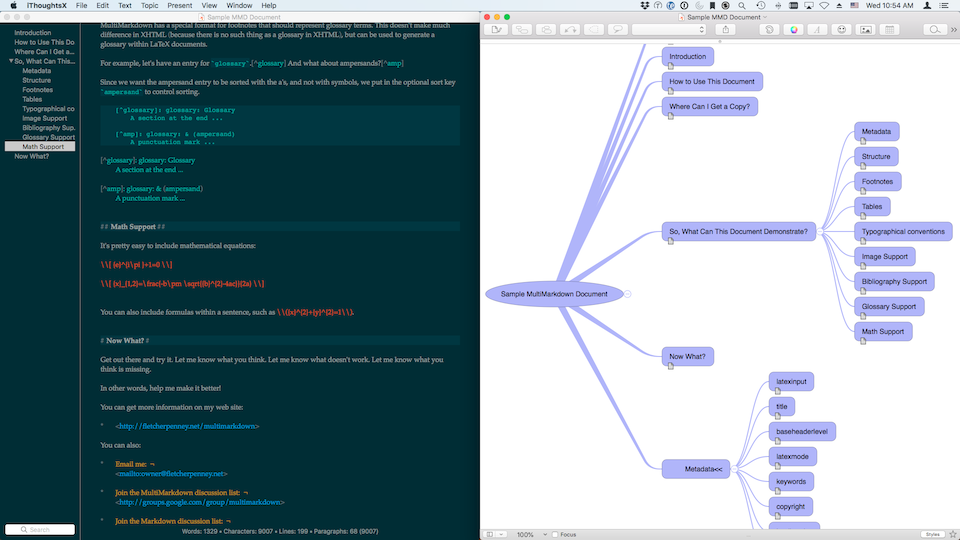
\includegraphics[keepaspectratio,width=\textwidth,height=0.75\textheight]{images/split-view.png}
\caption{Example of advanced use of the ITMZ format}
\end{figure}

\input{mmd6-tufte-book-footer}
\end{document}
